\documentclass[11pt]{article}

% Packages

\usepackage{amsmath, amsfonts, amssymb, amsthm}
\usepackage{enumitem}
\usepackage{mathtools}
\usepackage{natbib}
\usepackage{graphicx}
\usepackage{hyperref}
\usepackage{cleveref}
\usepackage{graphicx}

\newcommand{\defaultindent}{\hspace{15pt}}
\newcommand{\subsectionindent}{\hspace{30pt}}
\newcommand{\subsubsectionindent}{\hspace{15pt}}

\newcommand{\expectation}{\mathrm{E}}
\newcommand{\variance}{\mathrm{Var}}

% Page Setup
\usepackage{fancyhdr}
            \setlength{\parindent}{0pt}
			\setlength{\headheight}{0.75in}
			\setlength{\oddsidemargin}{0in}
			\setlength{\evensidemargin}{0in}
			\setlength{\voffset}{-1.0in}
			\setlength{\headsep}{10pt}
			\setlength{\textwidth}{6.5in}
			\setlength{\headwidth}{6.5in}
			\setlength{\textheight}{8.75in}
			\setlength{\parskip}{1ex plus 0.5ex minus 0.2ex}
			\setlength{\footskip}{0.3in}
				\renewcommand{\headrulewidth}{0.5pt}
				\renewcommand{\footrulewidth}{0.0pt}
				\pagestyle{fancy}
				\lhead{}
				\chead{Probability and Statistics Coursework}
				\rhead{\nouppercase{\leftmark}}
				\lfoot{}
				\cfoot{\thepage}
				\rfoot{}
				
\title{Probability and Statistics
       \\ Coursework}
\author{}

\begin{document}

\maketitle




\section*{\centerline{Question 1}}


\subsection*{\subsectionindent (a)}

We have that: 
\begin{align*}
\expectation \left[ \overline{W} \right] & = \expectation \left[ \frac{1}{n} \sum_{i = 1}^{n} \frac{ g(X_i) }{ f(X_i) } \right] 
= \frac{1}{n} \expectation \left[ \sum_{i = 1}^{n} \frac{ g(X_i) }{ f(X_i) } \right]
= \frac{1}{n} \sum_{i = 1}^{n} \expectation \left[ \frac{ g(X_i) }{ f(X_i) } \right]
= \frac{1}{n} \sum_{i = 1}^{n} \expectation \left[ \frac{ g(X) }{ f(X) } \right]
= \frac{1}{n} \, n \, \expectation \left[ \frac{ g(X) }{ f(X) } \right]
\\                                       & = \expectation \left[ \frac{ g(X) }{ f(X) } \right]
= \int_{- \infty}^{+ \infty} \frac{ g(x) }{ f(x) } f(x) \, dx = \int_{- \infty}^{+ \infty} g(x) \, dx = I
\end{align*}
which implies that the sample mean of the weights is an unbiased estimator of the integral $I$.


\subsection*{\subsectionindent (b)}

Notice that: 
\[
\variance \left[ \frac{ g(X) }{ f(X) } \right] 
= \expectation \left[ \left( \frac{ g(X) }{ f(X) } \right) ^ 2 \right] - \expectation \left[ \frac{ g(X) }{ f(X) } \right] ^ 2
= \expectation \left[ \left( \frac{ g(X) }{ f(X) } \right) ^ 2 \right] - I ^ 2
\]
Since $(X_i)_{i \in \overline {1,n}}$ are i.i.d. we have that
\begin{align*}
\variance \left[ \overline{W} \right] & = \variance \left[ \frac{1}{n} \sum_{i = 1}^{n} \frac{ g(X_i) }{ f(X_i) } \right]
= \frac{1}{n^2} \variance \left[ \sum_{i = 1}^{n} \frac{ g(X_i) }{ f(X_i) } \right]
= \frac{1}{n^2} \sum_{i = 1}^{n} \variance \left[ \frac{ g(X_i) }{ f(X_i) } \right]
= \frac{1}{n^2} \sum_{i = 1}^{n} \variance \left[ \frac{ g(X) }{ f(X) } \right]
\\                                    & = \frac{1}{n^2} \, n \, \variance \left[ \frac{ g(X) }{ f(X) } \right]
= \frac{1}{n} \variance \left[ \frac{ g(X) }{ f(X) } \right]
= \frac{1}{n} \left( \expectation \left[ \left( \frac{ g(X) }{ f(X) } \right) ^ 2 \right] - I ^ 2 \right)
\end{align*}
which implies that the variance of the estimator $\overline{W}$ is proportional to $\left( \expectation \left[ \left( \frac{ g(X) }{ f(X) } \right) ^ 2 \right] - I ^ 2 \right)$.

The standard deviation of $\overline{W}$ is given by :
\[ \sigma_{\overline{W}} 
= \sqrt{\variance \left[ \overline{W} \right]} 
= \frac{1}{\sqrt{n}} \cdot \sqrt{ \expectation \left[ \left( \frac{ g(X) }{ f(X) } \right) ^ 2 \right] - I ^ 2 }
\]
We have $2$ cases:

\medskip 

\quad \underline{Case $1$}: $\expectation \left[ \left( \frac{ g(X) }{ f(X) } \right) ^ 2 \right] - I ^ 2 = 0$

Then the standard deviation $\sigma_{\overline{W}}$ is equal to $0$ regardless of the value of $n$. 

\medskip

\quad \underline{Case $2$}: $\expectation \left[ \left( \frac{ g(X) }{ f(X) } \right) ^ 2 \right] - I ^ 2 > 0$

Then the standard deviation of the estimator $\overline{W}$ scales proportional to $\frac{1}{\sqrt{n}} = n ^ { - \frac{1}{2} }$.


\subsection*{\subsectionindent (c)}

Suppose that $f(x) \propto g(x)$. That is, there is a constant $c \in \mathbb{R}$ such that $g(x) = c f(x)$.
\\ Then we have that: 
\[
\int_{- \infty}^{+ \infty} g(x) \, dx = I \Rightarrow \int_{- \infty}^{+ \infty} c f(x) \, dx = I \Rightarrow c \int_{- \infty}^{+ \infty} f(x) \, dx = I \Rightarrow c = I
\tag{since $X$ has pdf $f(x)$ } 
\]
which implies that
\[
\variance \left[ \overline{W} \right] 
= \frac{1}{n} \left( \expectation \left[ \left( \frac{ g(X) }{ f(X) } \right) ^ 2 \right] - I ^ 2 \right) 
= \frac{1}{n} \left( \expectation \left[ c ^ 2 \right] - I ^ 2 \right)
= \frac{1}{n} \left( c ^ 2 - I ^ 2 \right)
= \frac{1}{n} \left( I ^ 2 - I ^ 2 \right)
= 0
\]
Therefore the variance of the estimator is $0$, which implies that $f(x) \propto g(x)$ is the ideal choice for the RV $X$. But this choice is impractical to use since the constant of proportionality needed is $I$ itself. (which is the quantity that we want to estimate)


\subsection*{\subsectionindent (d)}

In order to compute the \textbf{estimate} using samples from $N(0,\sigma ^ 2)$, we use the following algorithm: 

\quad \textit{\underline{Step $1$}}: \textit{Generate a sample of size} $n = 20$ \textit{from} $N(0,1)$.

This can be done using \verb+numpy.random.randn()+.

\quad \textit{\underline{Step $2$}}: \textit{Multiply every value by} $\sigma$. \textit{Then we get a sample of size} $n = 20$ \textit{from} $N(0,\sigma ^ 2)$.

\quad \textit{\underline{Step $3$}}: \textit{Apply the function} $x \to \frac{ g(x) }{ \text{pdf of } N(0,\sigma ^ 2)}$ \textit{to every element of the sample}. 

In this way, we obtain the weights needed to estimate the integral.

\quad \textit{\underline{Step $4$}}: \textit{Compute the sample mean of the weights.} Then this will be an estimation of the integral.

This can be done by using \verb+numpy.mean()+.

\medskip

In order to compute the \textbf{confidence interval} for our estimation, we need to use a Student’s $t$-distribution, as we are assuming that the weights are normally
distributed (we know the mean of the normal distribution = the mean of the weights, but we don't know the standard deviation).

By computing the standard error mean, we can use the formula for a $100(1 - \alpha) \% $ confidence interval for $I$ in order to get the desired result.

Alternatively, this can be done by using \verb+scipy.stats.t.interval()+.


\rule{\textwidth / 2}{0.4pt}

In the given case, we obtain the following result:

    estimate of the integral:  $1.6936228751468119$
\\  $95\%$ confidence interval:  $(1.1776665653117973, 2.2095791849818265)$


\subsection*{\subsectionindent (e)}

The list of values of $\sigma$ is $[0.5, 1.0, 1.5, 2.0, 2.5, 3.0, 3.5, 4.0, 4.5, 5.0]$.

For every $\sigma$ in the given list, we apply the previous $2$ algorithms in order to get the estimation and confidence interval. Then we plot those in figure with $\sigma$ on the $x$-axis and $I$ on the $y$-axis.

Moreover, we also add a horizontal line to the plot at the true value of $I = 1.81280$.

\begin{figure}[h]
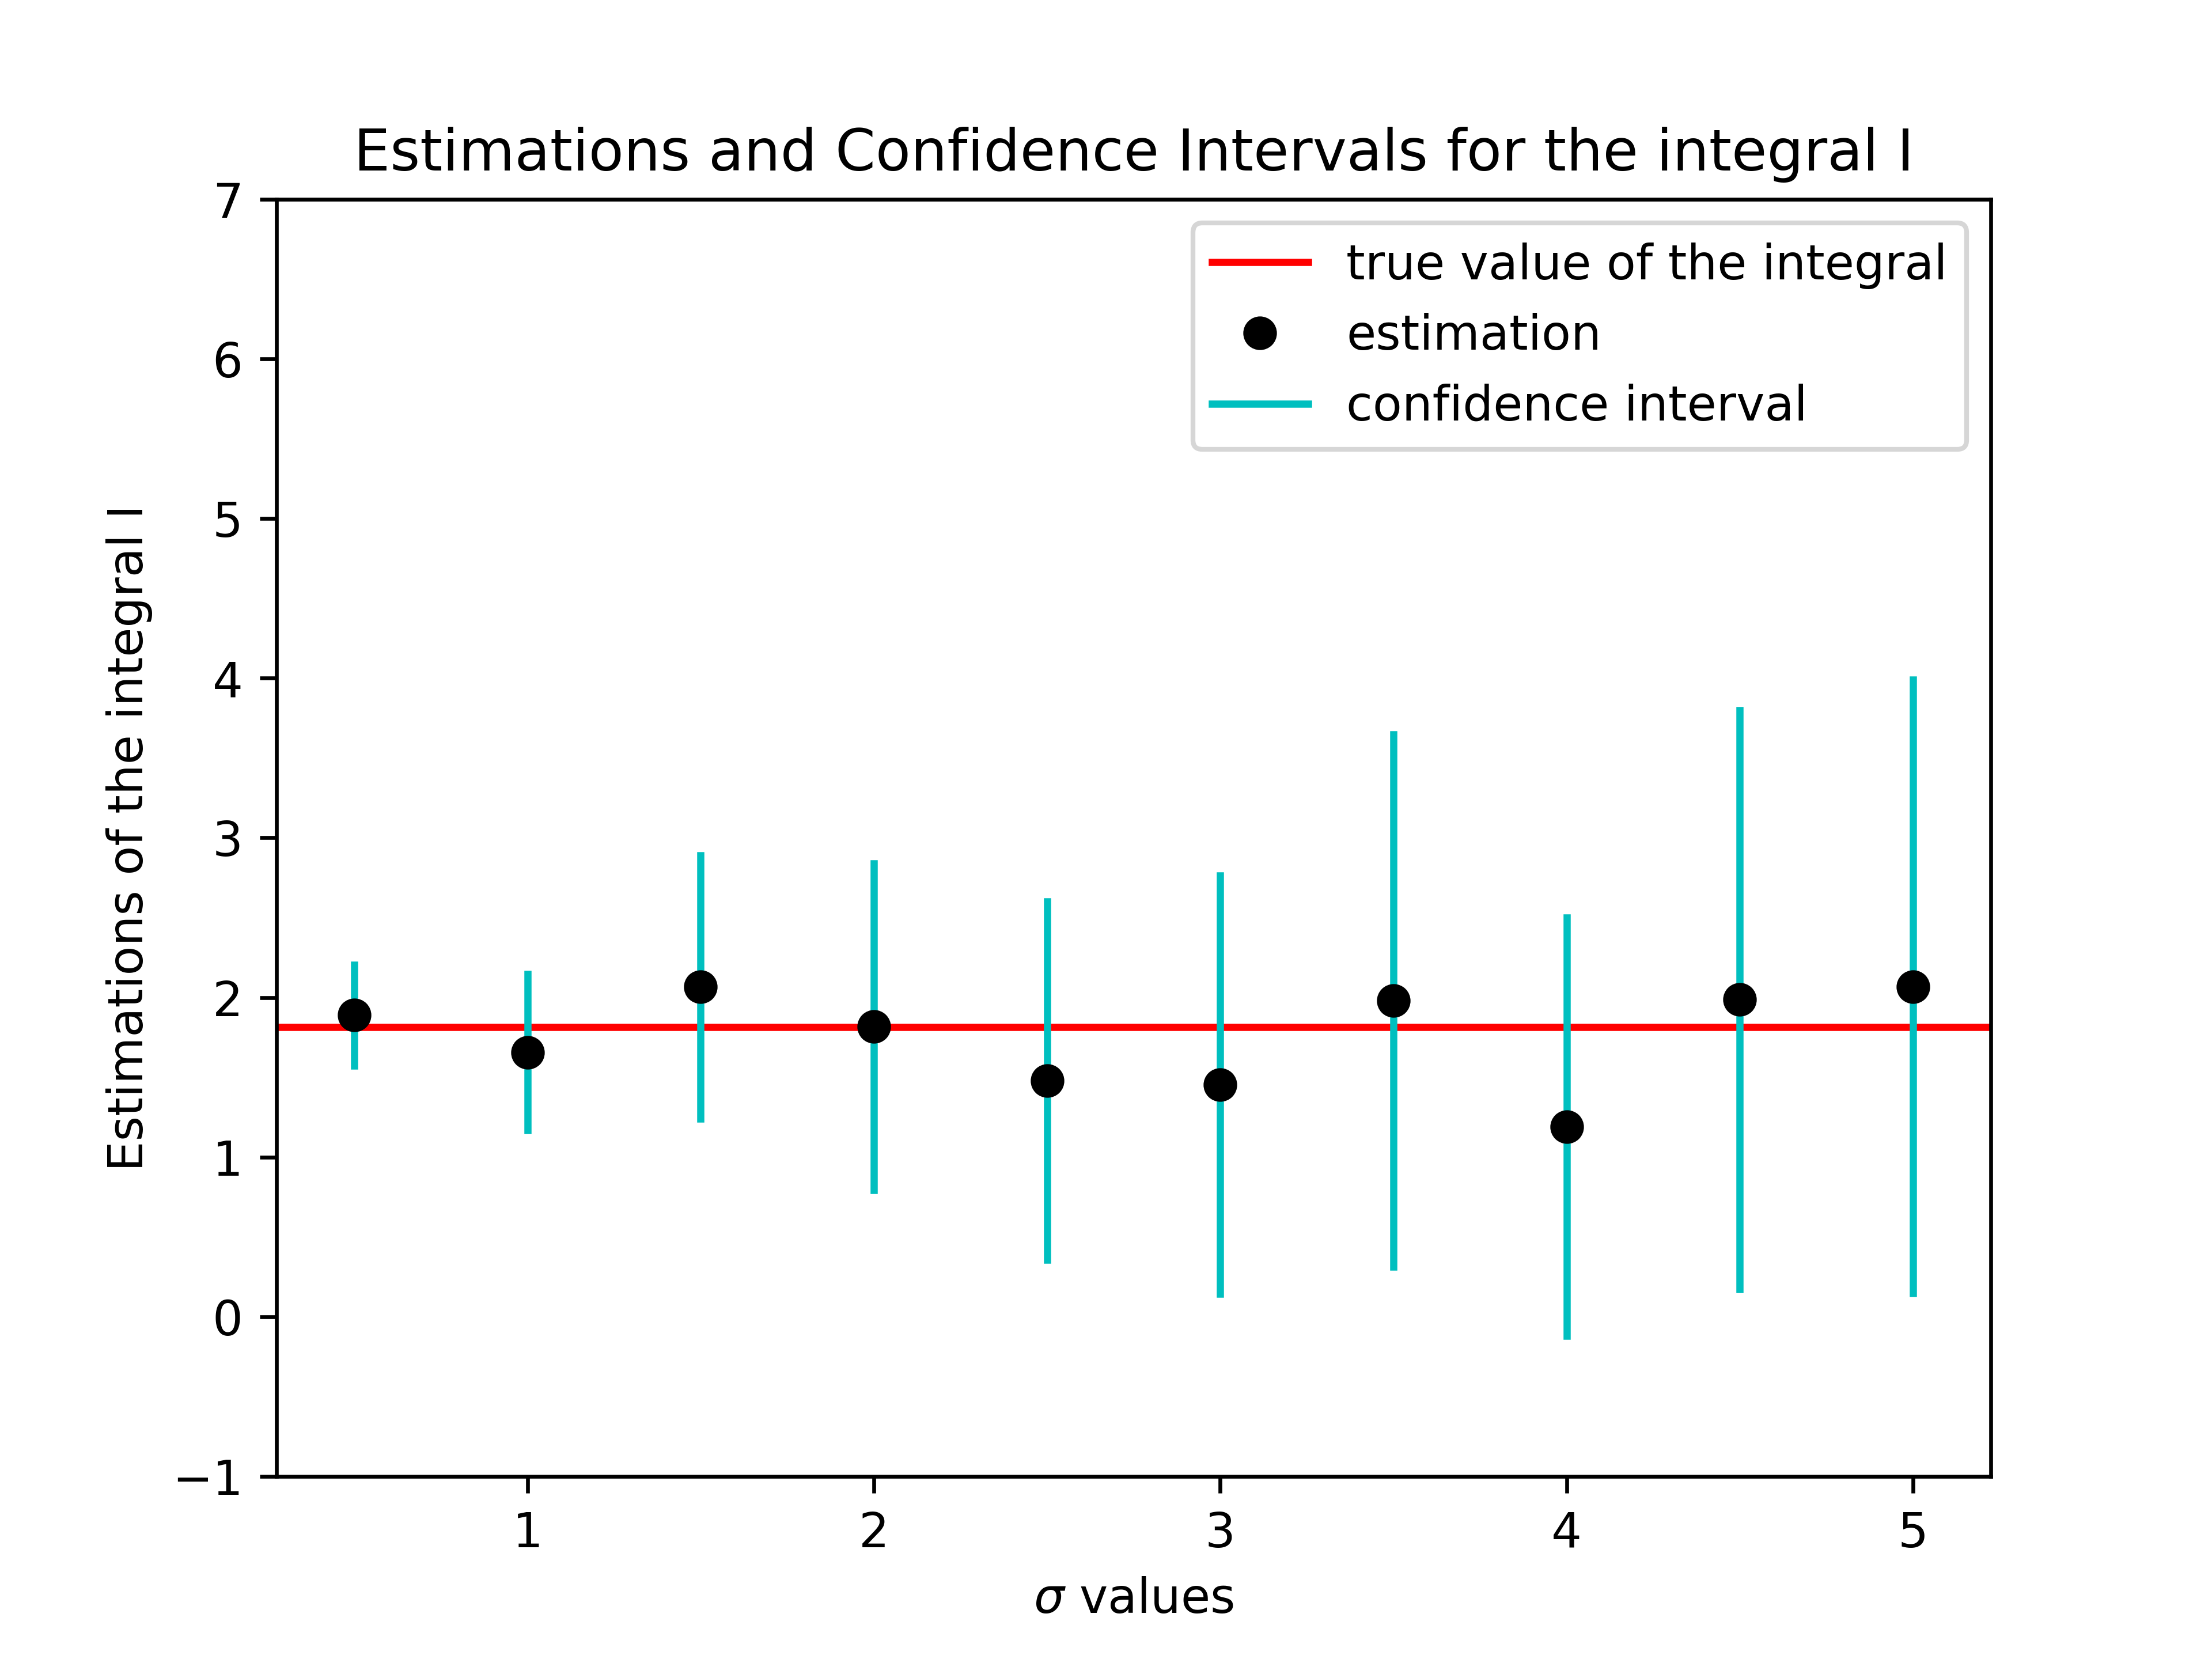
\includegraphics[width=12cm]{submission/question1_e}
\centering
\end{figure}

\subsection*{\subsectionindent (f)}

For each $n$ in $[2^3, 2^4, ... , 2^{12}]$, we repeat the experiments $100$ times and get $100$ estimations of the integral. Then we compute the standard deviation of these estimations by using \verb+numpy.std()+.

At part \textbf{(b)}, we predicted that the standard deviation scales as $n ^ { - \frac{1}{2} }$. We then plot the line $y = \sigma_{n = 8} \left( \frac{n}{8} \right) ^ {\lambda}$, where $\sigma_{n = 8}$ is the standard deviation of the $100$ estimates for the $n = 8$ case and $\lambda = - \frac{1}{2}$ .

The log-log plot was constructed using \verb+matplotlib.pyplot.loglog()+.

\newpage

\begin{figure}[h]
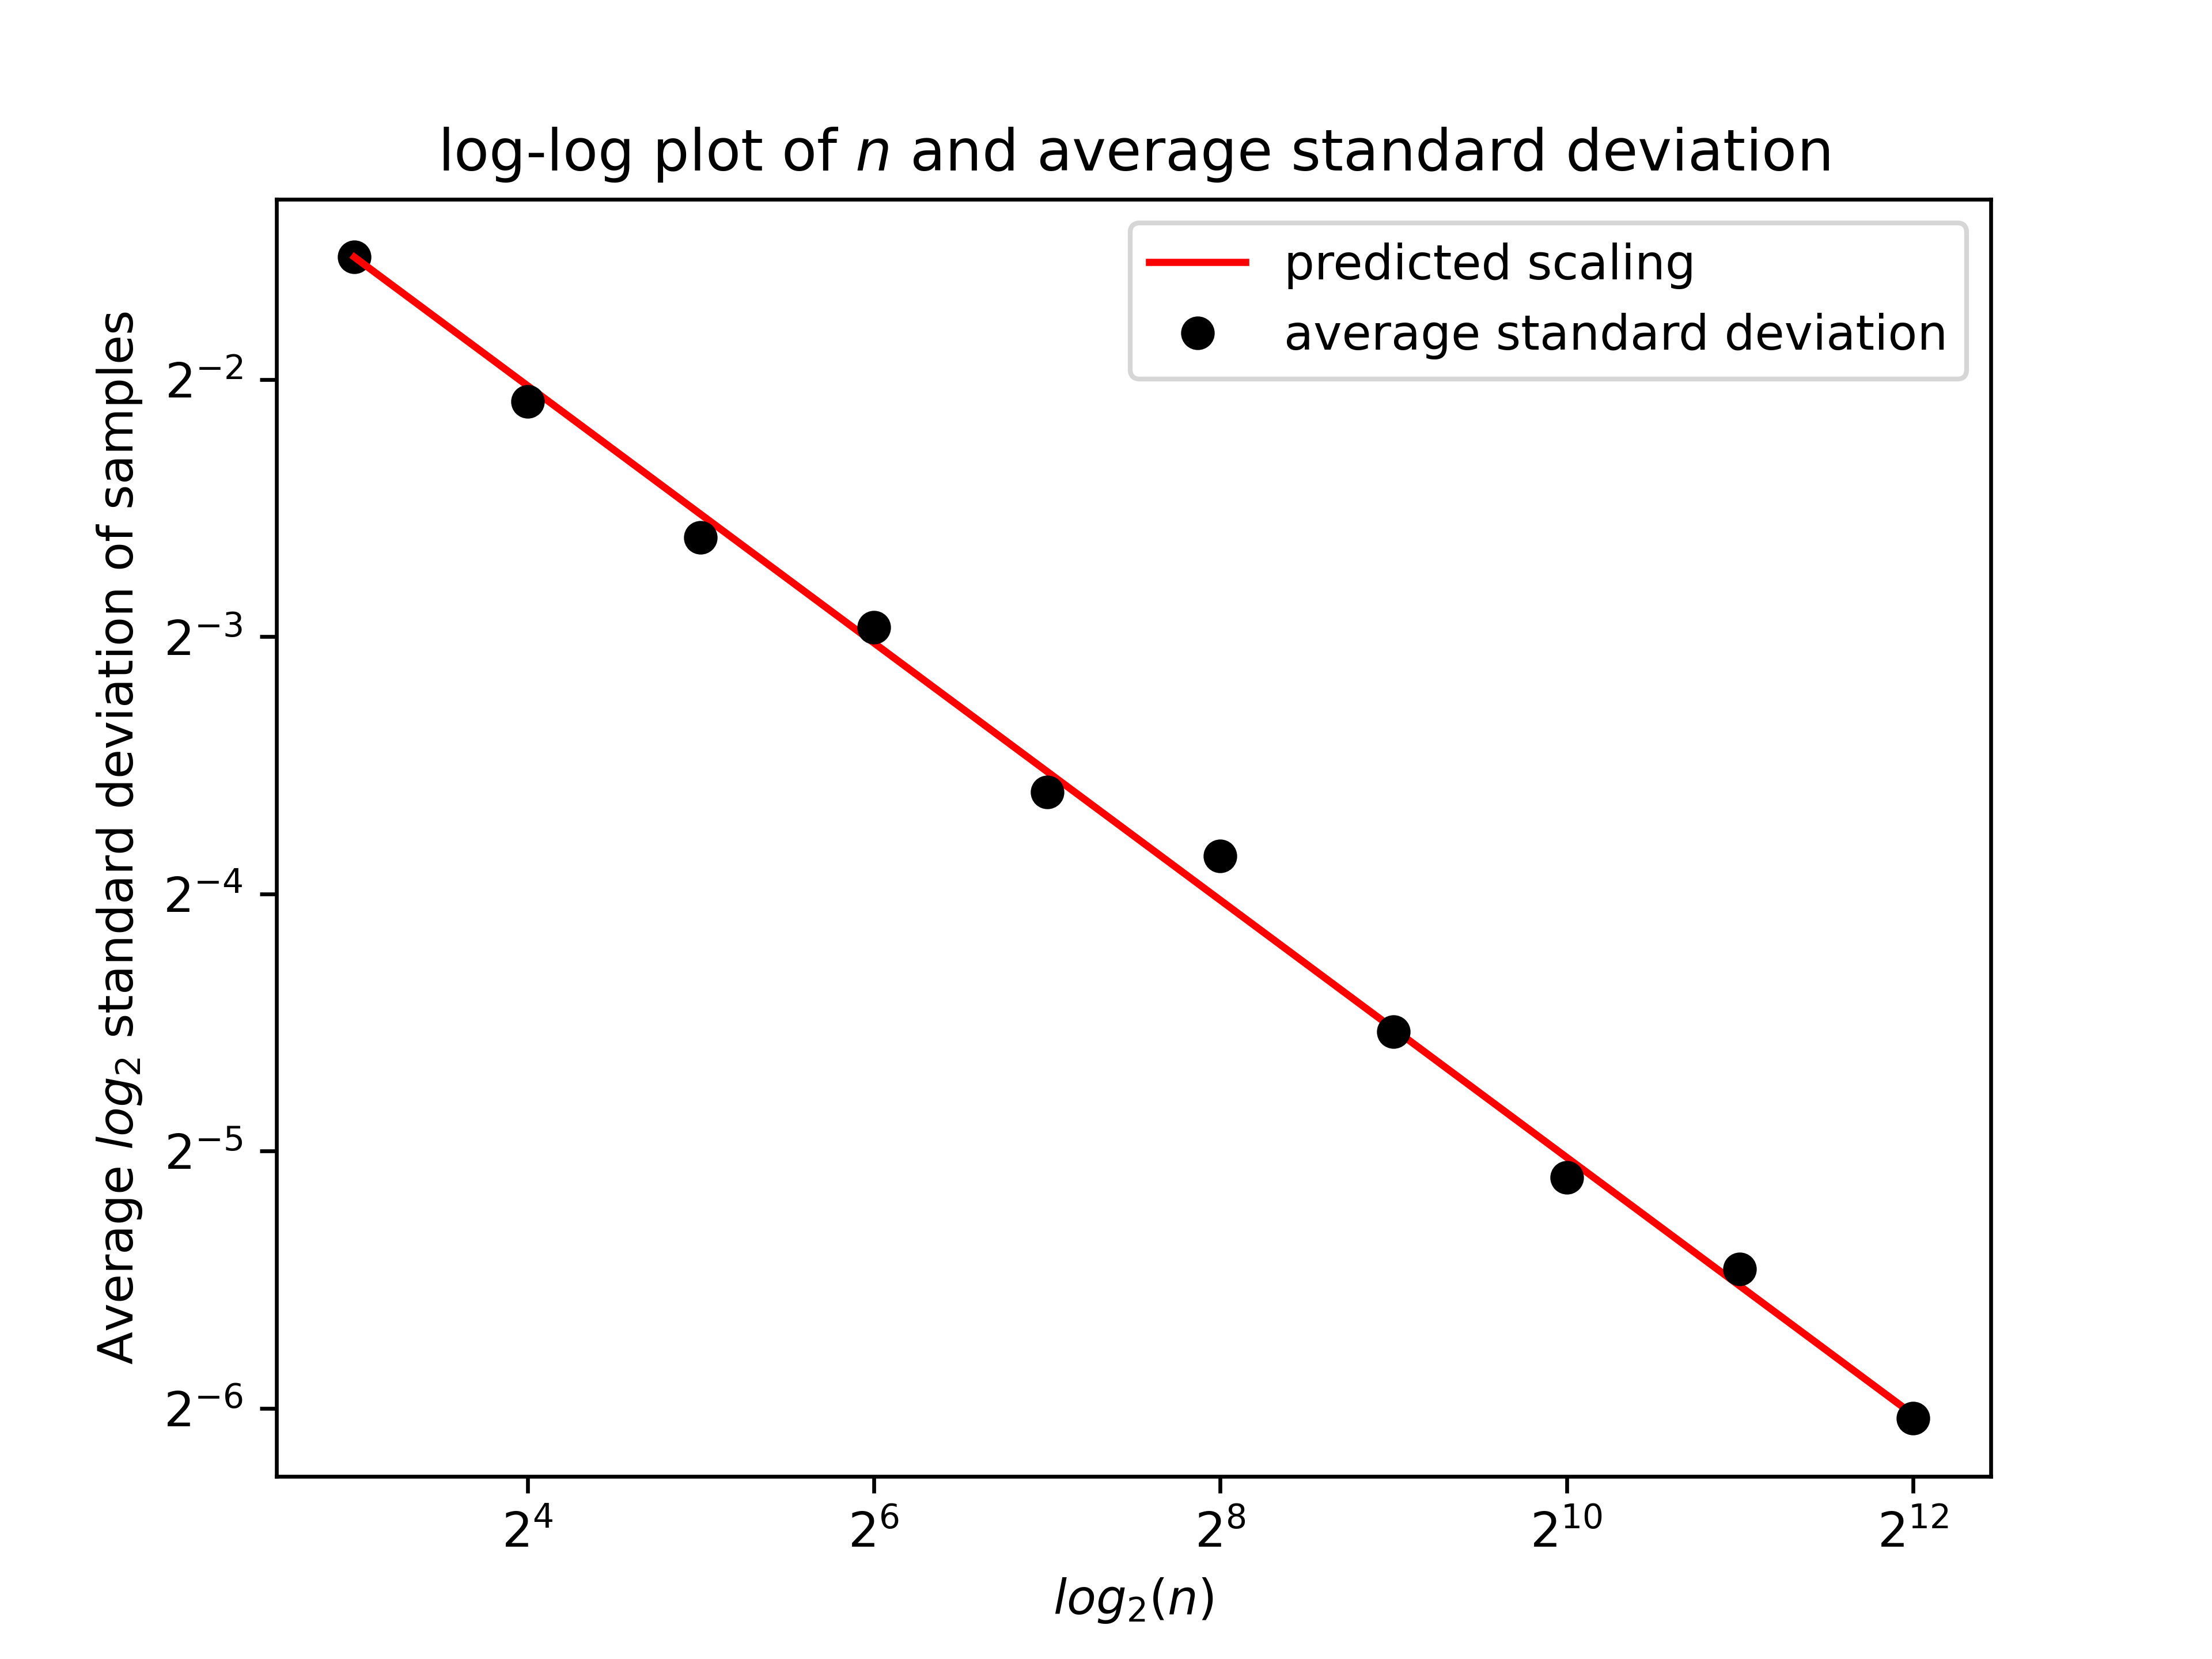
\includegraphics[width=12cm]{submission/question1_f}
\centering
\end{figure}

\subsection*{\subsectionindent (g)}

The standard deviation of the random variable $X$ is given by:
\[
\sigma = \sigma_X = \sqrt{ \expectation \left[ \left( \frac{ g(X) }{ f(X) } \right) ^ 2 \right] - I ^ 2 }
\] 

The standard deviation of the estimator is given by 
\[
\sigma_{\overline{W}}  = \frac{1}{\sqrt{n}} \cdot \sqrt{ \expectation \left[ \left( \frac{ g(X) }{ f(X) } \right) ^ 2 \right] - I ^ 2 } = \frac{1}{\sqrt{n}} \, \cdot \,\sigma_X
\]

In order for the estimator to be a good one, it needs to have a low standard deviation (otherwise it can give us values which are far from the true value of the integral $I$). If the pdf $f(x)$ is much “narrower” or “broader” than $g(x)$, then the standard deviation of the random variable $X$ is a large number. Thus, if we want to estimate $g(x)$ using $f(x)$, we will need a large number of samples.

\defaultindent But this make the algorithm impractical to use, since for a given case, we don't know how many samples we need in order for the estimator to have a low standard deviation.


\newpage

\section*{\centerline{Question 2}}

For every $x \in \mathbb{R}$, we have that: 
\begin{align*}
F_X (x) & = P ( X \le x ) 
= P ( F^{-1} (U) \le x ) 
= P ( U \le F(x) ) 
\tag{since $F$ is increasing } 
\\      & = F(x) 
\tag{since $\forall y \in \mathbb{R} , 0 \le F(y) \le 1$ and $U \sim U(0,1)$ } 
\end{align*}
which implies that the cdf of $X$ is $F(x)$.




\section*{\centerline{Question 3}}


\subsection*{\subsectionindent (a)}

Since $f_X ( x )$ is a pdf, we have that $\int_{- \infty}^{\infty} f_X ( x ) \, dx = 1$.
\begin{align*}
\int_{- \infty}^{\infty} f_X ( x ) \, dx = 1 & \Rightarrow \int_{ x_{ min } }^{\infty} c \cdot \left( \frac{x}{x_{min}} \right) ^ {- \lambda} \, dx = 1 
\tag{by the definition of $f_X (x)$ }
\\                                           & \Rightarrow c \cdot \frac{1}{ x_{min}^{- \lambda}} \cdot \left[ \frac{x ^ {- \lambda + 1}}{- \lambda + 1} \right]_{x = x_{min}}^{x = \infty} = 1 
\Rightarrow c \cdot \frac{1}{ x_{min}^{- \lambda}} \cdot \left[ 0 - \frac{x_{min} ^ {- \lambda + 1}}{- \lambda + 1} \right] = 1
\\                                           & \Rightarrow c \cdot \frac{x_{min}}{- \lambda + 1} = - 1 \Rightarrow c = \frac{\lambda - 1}{x_{min}}
\end{align*}
Thus $c = \frac{\lambda - 1}{x_{min}}$. 


\subsection*{\subsectionindent (b)}

Let \underbar{$x$} $ = (x_1, \dots , x_n)$ be the measured massed of the $n$ galaxies.

The log-likelihood is given by: 
\[
\ell (\lambda, \underbar{$x$}) = \sum_{i = 1}^{n} \log [ f_{X | \lambda} (x_i) ] 
= \sum_{i = 1}^{n} \log [ ( \lambda - 1 ) \cdot x_i^{- \lambda} ] 
= n \cdot log (\lambda - 1) - \lambda \cdot \sum_{i = 1}^{n} \log (x_i) 
\]
For every $i \in \overline{1,n}$, we have that $x_i \ge 1$, which implies that $\sum_{i = 1}^{n} \log (x_i) \ge 0$.

\medskip 

\quad \underline{Case $1$}: $\sum_{i = 1}^{n} \log (x_i) > 0$ 

We differentiate $\ell (\lambda, \underbar{$x$})$:
\[
\frac{\partial}{\partial \lambda} \ell (\lambda, \underbar{$x$}) = \frac{n}{\lambda - 1} - \sum_{i = 1}^{n} \log (x_i) 
\]
Setting this derivative equal to $0$, we get:
\[
\frac{n}{\hat{\lambda} - 1} - \sum_{i = 1}^{n} \log (x_i) = 0 
\Rightarrow \hat{\lambda} = 1 + \frac{n}{\sum_{i = 1}^{n} \log (x_i)}
\]
Now we find the second derivate of $\ell (\lambda, \underbar{$x$})$:
\[
\frac{\partial^2}{\partial^2 \lambda} \ell (\lambda, \underbar{$x$}) = \frac{ - n }{ (\lambda - 1)^2 }
\]
which is $< 0$ for every $\lambda > 1$. 

\defaultindent Therefore $\hat{\lambda} = 1 + \frac{n}{\sum_{i = 1}^{n} \log (x_i)}$ is the MLE for $\lambda$.

\medskip

\quad \underline{Case $2$}: $\sum_{i = 1}^{n} \log (x_i) = 0$  

Then the log-likelihood is given by: 
\[
\ell (\lambda, \underbar{$x$}) = n \cdot log (\lambda - 1) 
\]
In this case we don't have a MLE, since this function is defined on $(0,\infty)$ and is strictly increasing.


\subsection*{\subsectionindent (c)}

The pdf of the power law distribution is 
$ f_X (x) = 
            \begin{cases}
              (\lambda - 1) x^{- \lambda} & \text{, if } x \ge 1
              \\ 0                        & \text{, if } x < 1
            \end{cases}
$ 

For any $x < 1$, we have that $F_X (x) = 0$. 
\\ For any $x \ge 1$, we have that: 
\[
F_X (x) = \int_{- \infty}^{x} f_X ( t ) \, dt = \int_{1}^{x} f_X ( t ) \, dt 
= \int_{1}^{x} (\lambda - 1) t^{- \lambda} \, dt  
= (\lambda - 1) \left[ \frac{t ^ {- \lambda + 1}}{- \lambda + 1} \right]_{t=1}^{t=x}
= 1 - x^{- \lambda + 1}   
\]
Notice that $F_X ( \mathbb{R} ) = [0,1)$.
\\ \hspace*{\fill} [ since $F_X (x) = 0$ for every $x \le 1$ , $F_X$ is continuous and $\lim_{x \to \infty} F_X (x) = 1$ ] 
\\ For every $y \in (0,1)$, we have that $F_X ^{-1} ( \{ y \} ) = \{ (1 - y)^{\frac{1}{- \lambda + 1}} \}$. 
\\ \hspace*{\fill} [ since $1 - x^{- \lambda + 1} = y \Leftrightarrow x = (1 - y)^{\frac{1}{- \lambda + 1}}$ ]
\\ For $y = 0$, we have that $F_X ^{-1} ( \{ 0 \} ) = ( - \infty, 1]$.

\defaultindent Therefore the quartile function $Q : (0,1) \to (1, \infty)$ is given by 
\[
Q(y) = (1 - y)^{\frac{1}{1 - \lambda}} \text{ , for every } y \in (0,1)
\]


\subsection*{\subsectionindent (d)}

In order to generate this plot, I used the following algorithm:

\quad \textit{\underline{Step $1$}}: \textit{Generate} $n$ \textit{samples of} $U(0,1)$.

This can be done by using \verb+numpy.random.rand()+.

\quad \textit{\underline{Step $2$}}: \textit{Apply the quantile function ( with the parameter} $\lambda$ \textit{) to every sample from} $U(0,1)$.
 
Then we get the $n$ samples of $X$ when the true value of the parameter is $\lambda$.

\quad \textit{\underline{Step $3$}}: \textit{Compute} $\hat{\lambda}$ using the formula from \textbf{(b)}.

\quad \textit{\underline{Step $4$}}: \textit{Repeat this} $10^4$ \textit{times to get to get a sample} $(\hat{\lambda}_1, \hat{\lambda}_2, ... , \hat{\lambda}_{10 ^ 4})$. \textit{Then we create a density histogram from these} $10^4$ \textit{values}.

\newpage 

\begin{figure}[h]
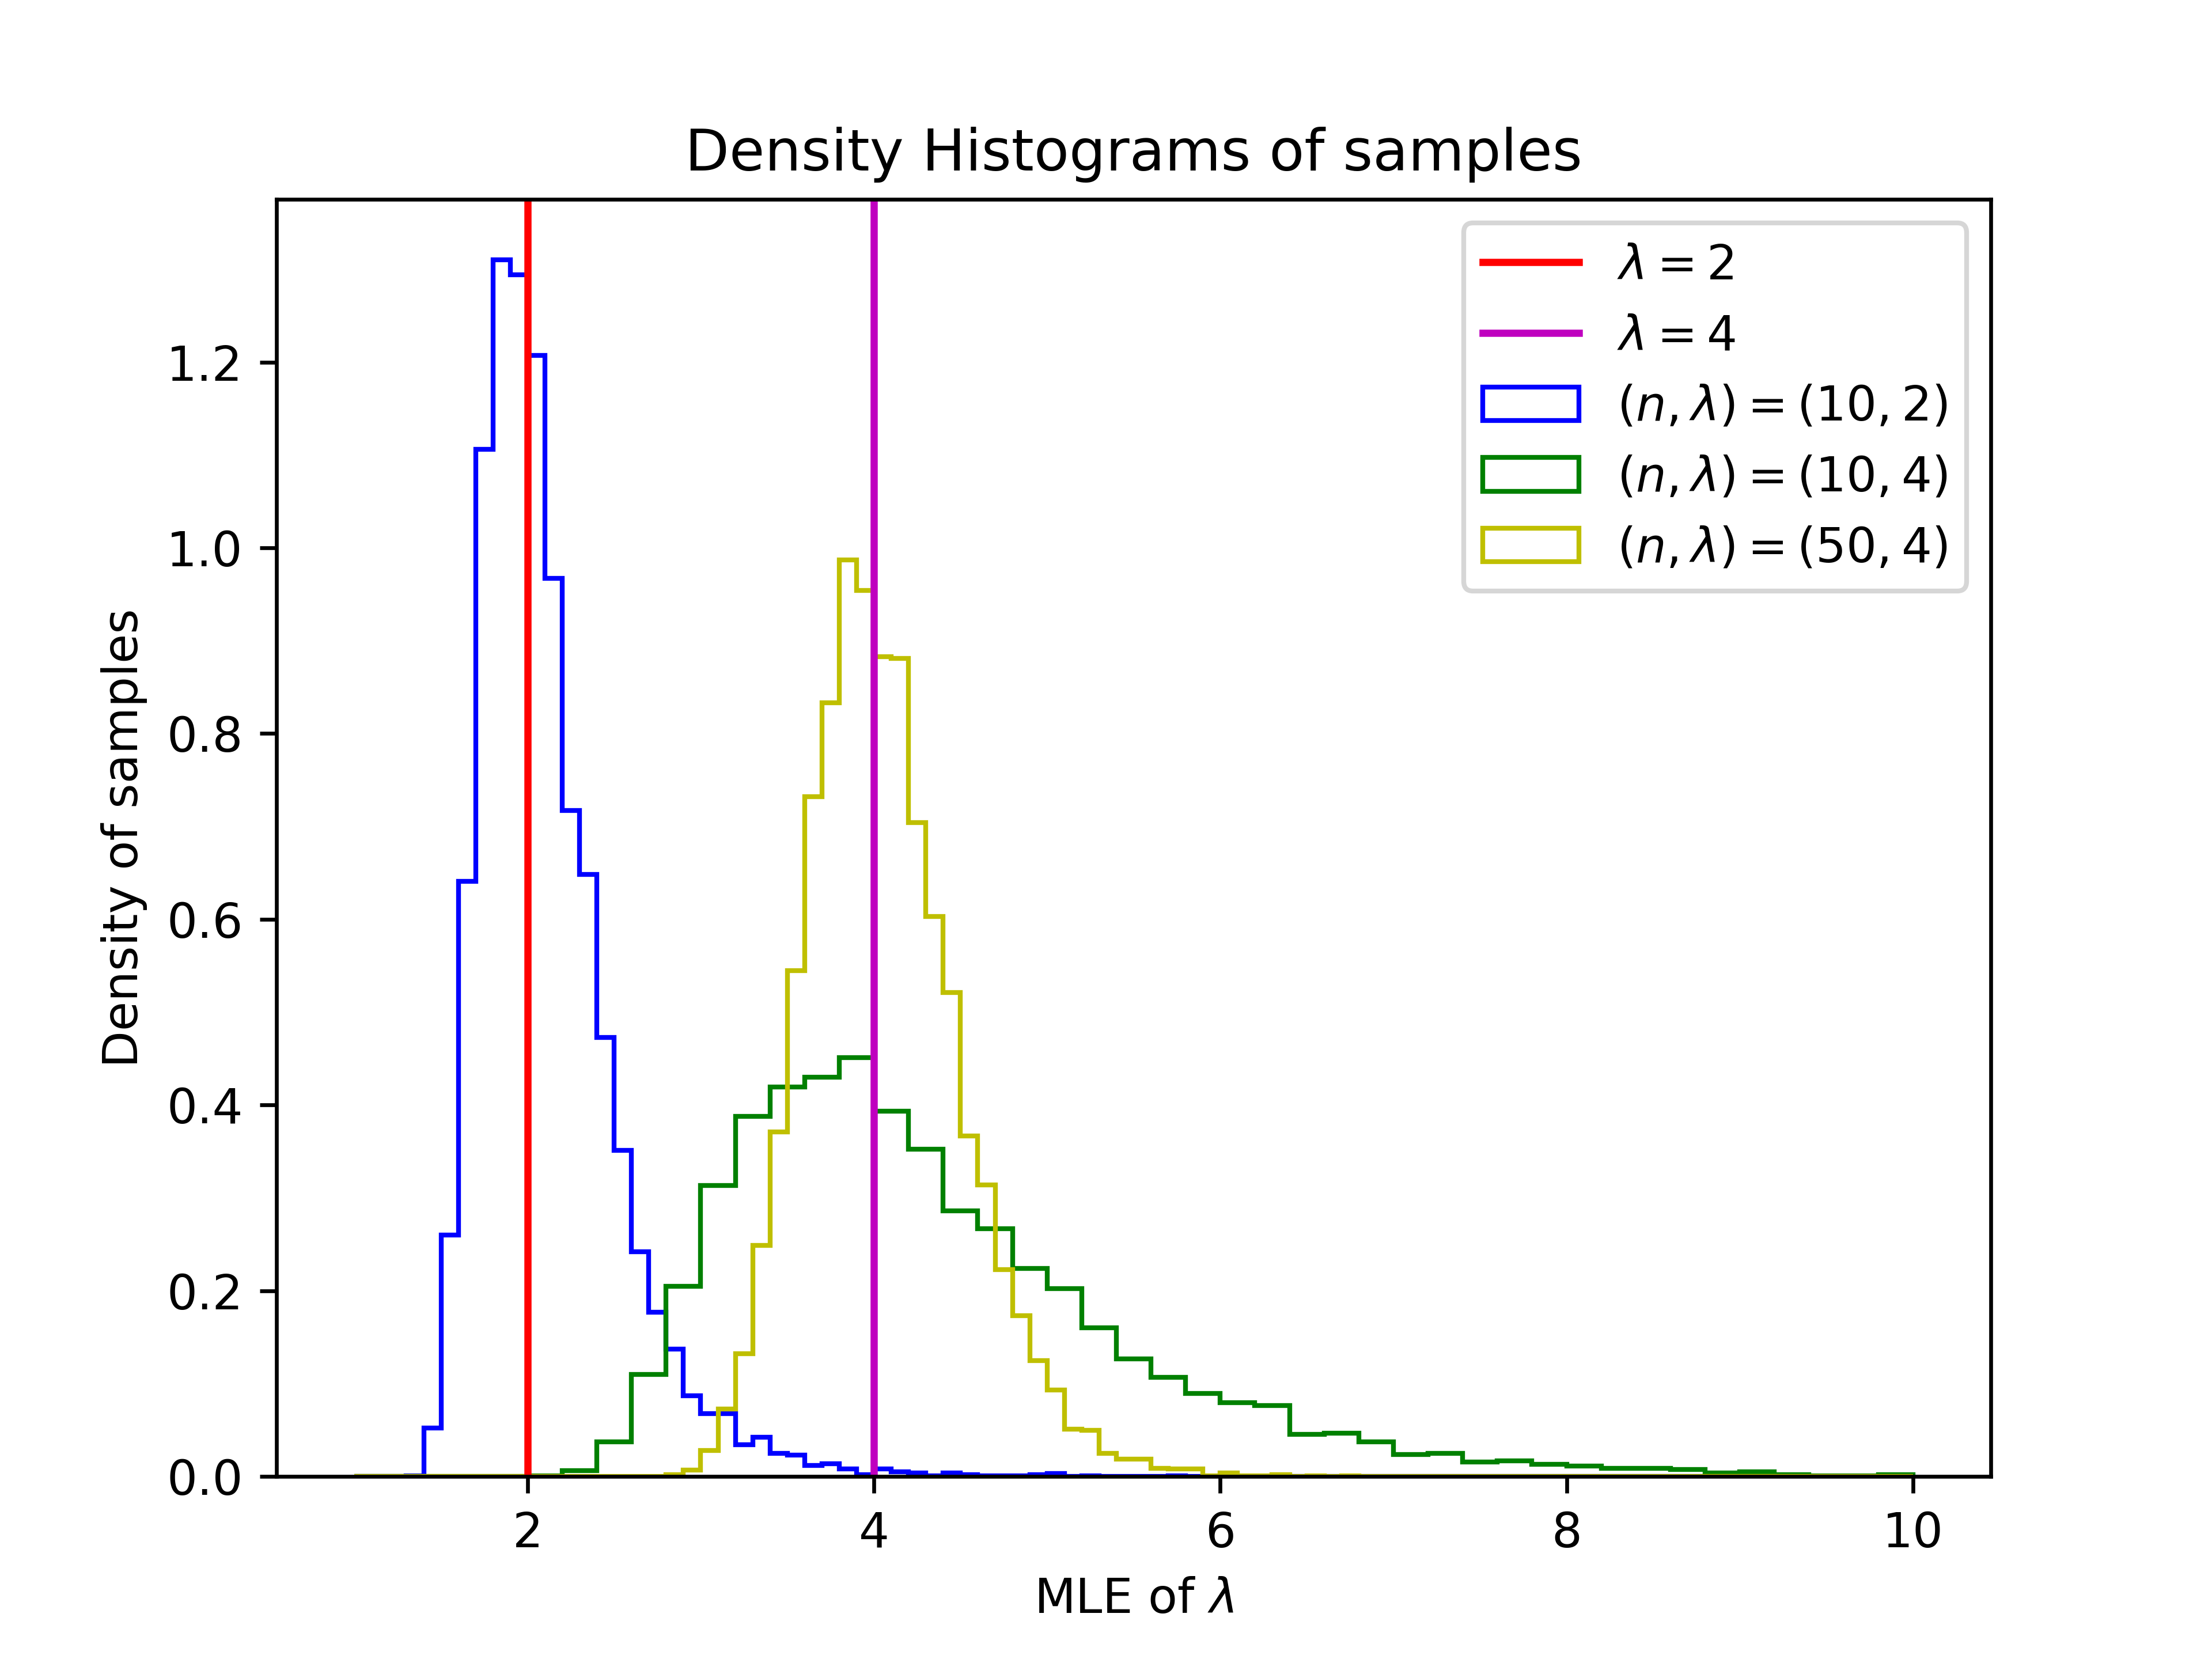
\includegraphics[width=14cm]{submission/question3_d}
\centering
\end{figure}

\subsection*{\subsectionindent (e)}

\defaultindent From now on, we will refer to the array corresponding to $(n, \lambda)$ as $\text{mle\_array\_} n \_ \lambda$.
\\ (And its sorted version will be referred as $\text{sorted\_mle\_array\_} n \_ \lambda$)

\subsubsection*{\subsubsectionindent (i)}

Our previous plot suggest that the rejection in this case should be a right-tailed one. 

In order to compute a right-tailed \textbf{rejection region} of an $\text{mle\_array}$, we use the following algorithm:

\quad \textit{\underline{Step $1$}}: \textit{Sort the MLE array.}

This can be done using \verb+numpy.sort()+.

We get the sorted array $\text{sorted\_mle\_array}$. Since the MLE array is now sorted, the empirical CDF is given by 
\begin{align*}
ECDF(x) & = \frac{\text{number of elements } \le x}{\text{length of the array}} 
\tag{\text{ECDF = empirical CDF}}
\\      & = \frac{\text{index of } x \text{ in sorted\_mle\_array} + 1}{\text{length of the array}}
\tag{assuming that the list index starts with $0$}
\end{align*}

\quad \textit{\underline{Step $2$}}: \textit{Compute} $\text{index} = \text{ceil} [ \alpha \cdot \text{length(mle\_array)} ] - 1$. 

Then this will satisfy:
\[
\text{ECDF (sorted\_mle\_array[index - 1])} < \alpha <= \text{ECDF (sorted\_mle\_array[index])}
\]
[$\text{sorted\_mle\_array[index]}$ will be the first element of the $\text{sorted\_mle\_array}$ which is $\ge \alpha$]

\quad \textit{\underline{Step $3$}}: \textit{The rejection region will be} $(\text{sorted\_mle\_array[index]}, + \infty)$.

\rule{\textwidth / 2}{0.4pt}

In the given case, we obtain the following result:

    Rejection region with Type I error $5\%$: $( 2.83779124447156 , + \infty )$

\subsubsection*{\subsubsectionindent (ii)}

In order to compute the \textbf{power} of the test, we use the following algorithm:

\quad \textit{\underline{Step $1$}}: \textit{Sort the} $\text{mle\_array\_} 10 \_ 4$.

This can be done using \verb+numpy.sort()+.

We get the sorted array $\text{sorted\_mle\_array\_} 10 \_ 4$.

\quad \textit{\underline{Step $2$}}: \textit{The rejection region is of the form} $(\text{rej}, + \infty)$. \textit{Find} index \textit{such that}:
\[
\text{sorted\_mle\_array}\_10\_4 [\text{index} - 1] < \text{rej} \le \text{sorted\_mle\_array}\_10\_4 [\text{index}]
\]
This can be done by using \verb+numpy.searchsorted()+.

\quad \textit{\underline{Step $3$}}: \textit{The power of the test is given by:}
\[
\text{power of the test} = \frac{ \text{length of mle\_array\_} 10 \_ 4 - \text{index} }{ \text{length of mle\_array\_} 10 \_ 4 }
\]
[$\text{length of mle\_array\_} 10 \_ 4 - \text{index}$ is the number of the elements of the $\text{mle\_array\_} 10 \_ 4$ that are in the rejection region]

 
\rule{\textwidth / 2}{0.4pt}

In the given case, we obtain the following result:

    The power of the test is:  $0.9638$

\subsubsection*{\subsubsectionindent (iii)}

In order to compute the \textbf{$p$-value} of an $\text{mle\_observation}$ (that is, MLE of an observation) given an $\text{mle\_array}$ (for which we assume that the rejection region is a right-tailed one),
\\we use the following algorithm:

\quad \textit{\underline{Step $1$}}: \textit{Sort the MLE array.}

This can be done using \verb+numpy.sort()+.

We get the sorted array $\text{sorted\_mle\_array}$.

\quad \textit{\underline{Step $2$}}: \textit{Find} index \textit{such that}:
\[
\text{sorted\_mle\_array} [\text{index} - 1] < \text{mle\_observation} <= \text{sorted\_mle\_array} [\text{index}]
\]
This can be done by using \verb+numpy.searchsorted()+.

\quad \textit{\underline{Step $3$}}: \textit{The} $p$-value \textit{is given by}:
\[
p\text{-value} = \frac{ \text{length of the mle\_array} - \text{index} }{ \text{length of the mle\_array} }
\]
[$\text{length of the mle\_array} - \text{index}$ is the number of the elements in $\text{mle\_array}$ which are $\ge \text{mle\_observation}$]

\rule{\textwidth / 2}{0.4pt}

In the given case, we obtain the following result:

    The MLE of this observation is:  $2.478118666755411$
\\  Since the MLE is not in the rejection region, there is insufficient evidence to reject null hypothesis at the $5\%$ level
\\  The $p$-value of this observation is:  $0.1419$ (that is, $14.19 \%$)


\end{document}       			